\documentclass[a4paper,11pt]{article}
\usepackage[utf8]{inputenc}
\usepackage[T1]{fontenc}
\usepackage{lmodern}
\usepackage[margin=1in]{geometry}
\usepackage{tikz}
\usetikzlibrary{shapes.geometric, arrows.meta, positioning, calc, fit, backgrounds}
\usepackage{xcolor}
\usepackage{hyperref}
\usepackage{tcolorbox}
\usepackage{booktabs}
\usepackage{graphicx}
\usepackage{enumitem}
\usepackage{titlesec}
\usepackage{microtype}

% Define brand colors
\definecolor{brandPrimary}{HTML}{1A3C5E}
\definecolor{brandAccent}{HTML}{2E86AB}
\definecolor{brandSuccess}{HTML}{22C55E}
\definecolor{brandSurface}{HTML}{1A1A2E}
\definecolor{brandDark}{HTML}{0F0F14}
\definecolor{brandGray}{HTML}{9090A0}

% Hyperlink styling
\hypersetup{
    colorlinks=true,
    linkcolor=brandAccent,
    filecolor=brandAccent,      
    urlcolor=brandAccent,
    pdftitle={Locara Atlas - MVP Architecture},
    pdfpagemode=FullScreen,
}

% Section styling
\titleformat{\section}{\Large\bfseries\color{brandPrimary}}{\thesection}{1em}{}[\titlerule]
\titleformat{\subsection}{\large\bfseries\color{brandAccent}}{\thesubsection}{1em}{}

% TikZ Styles
\tikzset{
    component/.style={rectangle, rounded corners, draw=brandPrimary, fill=brandPrimary!10, very thick, text width=3.5cm, align=center, minimum height=1.5cm, font=\sffamily\small},
    db/.style={cylinder, shape border rotate=90, aspect=0.25, draw=brandAccent, fill=brandAccent!10, very thick, text width=2.5cm, align=center, minimum height=1.5cm, font=\sffamily\small},
    client/.style={rectangle, rounded corners, draw=brandSuccess, fill=brandSuccess!10, very thick, text width=3cm, align=center, minimum height=1cm, font=\sffamily\small},
    arrow/.style={-{Stealth[scale=1.2]}, thick, draw=brandGray},
    biarrow/.style={{Stealth[scale=1.2]}-{Stealth[scale=1.2]}, thick, draw=brandGray},
    dashedarrow/.style={-{Stealth[scale=1.2]}, dashed, thick, draw=brandGray},
    tablebox/.style={rectangle, draw=brandPrimary, fill=white, thick, text width=4.5cm, font=\sffamily\scriptsize, rounded corners},
    tableheader/.style={fill=brandPrimary, text=white, font=\sffamily\scriptsize\bfseries, minimum height=0.6cm},
}

\begin{document}

\begin{titlepage}
    \centering
    \vspace*{4cm}
    {\Huge\bfseries\color{brandPrimary} Locara Atlas\par}
    \vspace{1cm}
    {\Large\bfseries Enterprise Dataset Delivery Platform\par}
    \vspace{2cm}
    {\large MVP Architecture \& Database Schema\par}
    \vspace{1.5cm}
    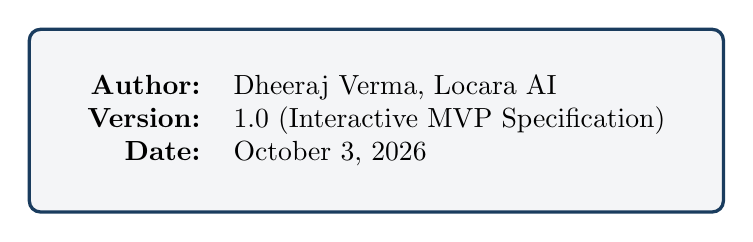
\begin{tikzpicture}
        \node[draw=brandPrimary, fill=brandPrimary!5, rounded corners, inner sep=15pt, very thick] {
            \begin{tabular}{rl}
                \textbf{Author:} & Dheeraj Verma, Locara AI \\
                \textbf{Version:} & 1.0 (Interactive MVP Specification) \\
                \textbf{Date:} & \today \\
            \end{tabular}
        };
    \end{tikzpicture}
    \vfill
    {\small \color{brandGray} Interactive Technical Specification Document\par}
\end{titlepage}

\tableofcontents
\newpage

\section{System Architecture Overview}
The Locara Atlas architecture is strictly decoupled to ensure the application remains lightning-fast even with 100,000+ videos. 

\begin{center}
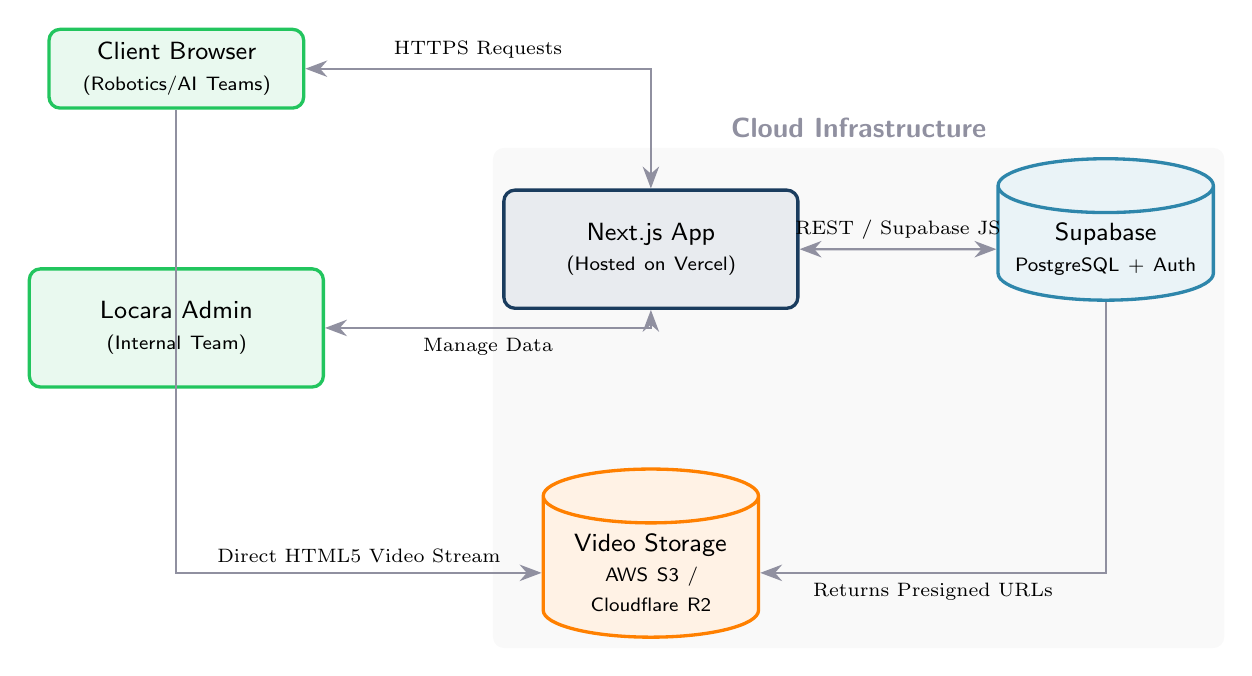
\begin{tikzpicture}[node distance=2cm and 2.5cm]
    % Nodes
    \node[client] (browser) {Client Browser \\ \scriptsize (Robotics/AI Teams)};
    
    \node[component, below right=of browser, yshift=1cm] (vercel) {Next.js App \\ \scriptsize (Hosted on Vercel)};
    
    \node[db, right=of vercel] (supabase) {Supabase \\ \scriptsize PostgreSQL + Auth};
    
    \node[component, below=of browser, fill=brandSuccess!10, draw=brandSuccess] (admin) {Locara Admin \\ \scriptsize (Internal Team)};
    
    \node[db, fill=orange!10, draw=orange, below=of vercel] (s3) {Video Storage \\ \scriptsize AWS S3 / Cloudflare R2};

    % Edges
    \draw[biarrow] (browser) -| node[pos=0.25, above, font=\scriptsize] {HTTPS Requests} (vercel);
    \draw[biarrow] (admin) -| node[pos=0.25, below, font=\scriptsize] {Manage Data} (vercel);
    
    \draw[biarrow] (vercel) -- node[above, font=\scriptsize] {REST / Supabase JS} (supabase);
    
    \draw[arrow] (browser) |- node[pos=0.75, above, font=\scriptsize] {Direct HTML5 Video Stream} (s3);
    
    \draw[arrow] (supabase) |- node[pos=0.75, below, font=\scriptsize] {Returns Presigned URLs} (s3);
    
    % Grouping
    \begin{scope}[on background layer]
        \node[fill=gray!5, rounded corners, fit=(vercel)(supabase)(s3), label={[font=\sffamily\bfseries, text=brandGray]above:Cloud Infrastructure}] {};
    \end{scope}
\end{tikzpicture}
\end{center}

\textbf{Critical Architecture Decision:} Video files (MP4s) are never stored inside the Next.js application, nor are they proxied through the server. The Supabase PostgreSQL database only stores the \texttt{video\_url}. The client browser fetches the metadata from Supabase via Next.js, and then directly streams the massive video files from the S3/R2 storage bucket.

\newpage
\section{Database ER Diagram (Supabase PostgreSQL)}

The backend strictly enforces tenant isolation via Row-Level Security (RLS). Below is the relational schema linking clients (organizations) to their assigned datasets.

\vspace{1cm}
\begin{center}
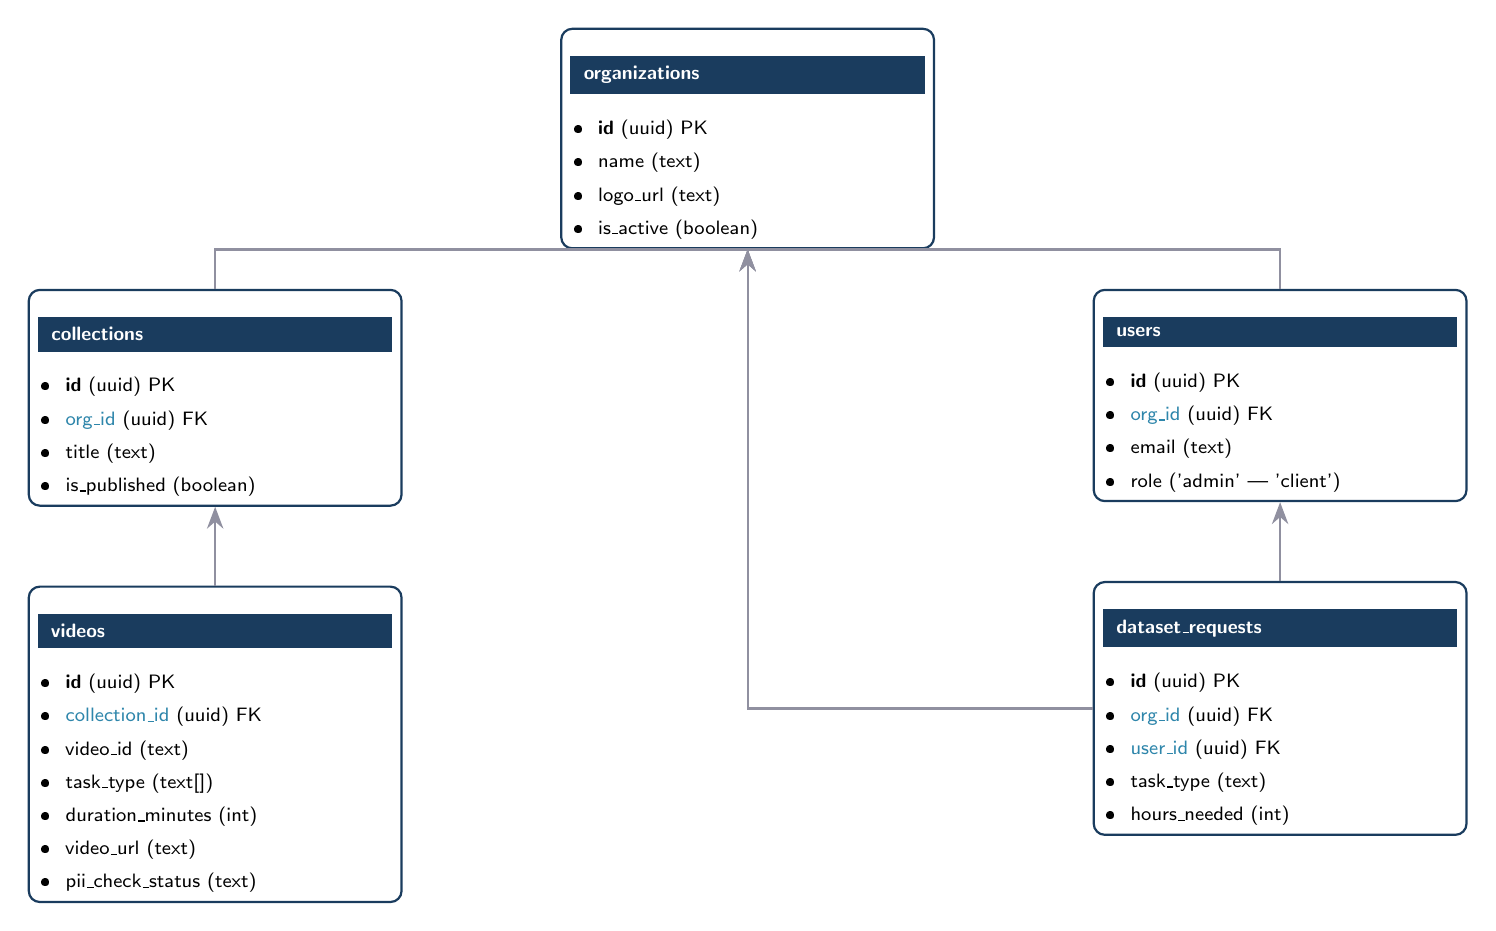
\begin{tikzpicture}[node distance=1.5cm and 2cm]

    % Organizations
    \node[tablebox] (org) {
        \begin{tcolorbox}[colback=brandPrimary, coltext=white, boxrule=0pt, arc=0pt, outer arc=0pt, top=1pt, bottom=1pt, left=2pt]
        \textbf{organizations}
        \end{tcolorbox}
        \vspace{-5pt}
        \begin{itemize}[leftmargin=10pt, itemsep=0pt]
            \item \textbf{id} (uuid) PK
            \item name (text)
            \item logo\_url (text)
            \item is\_active (boolean)
        \end{itemize}
    };

    % Users
    \node[tablebox, below right=of org, yshift=1cm] (users) {
        \begin{tcolorbox}[colback=brandPrimary, coltext=white, boxrule=0pt, arc=0pt, outer arc=0pt, top=1pt, bottom=1pt, left=2pt]
        \textbf{users}
        \end{tcolorbox}
        \vspace{-5pt}
        \begin{itemize}[leftmargin=10pt, itemsep=0pt]
            \item \textbf{id} (uuid) PK
            \item \textcolor{brandAccent}{org\_id} (uuid) FK
            \item email (text)
            \item role ('admin' | 'client')
        \end{itemize}
    };

    % Collections
    \node[tablebox, below left=of org, yshift=1cm] (coll) {
        \begin{tcolorbox}[colback=brandPrimary, coltext=white, boxrule=0pt, arc=0pt, outer arc=0pt, top=1pt, bottom=1pt, left=2pt]
        \textbf{collections}
        \end{tcolorbox}
        \vspace{-5pt}
        \begin{itemize}[leftmargin=10pt, itemsep=0pt]
            \item \textbf{id} (uuid) PK
            \item \textcolor{brandAccent}{org\_id} (uuid) FK
            \item title (text)
            \item is\_published (boolean)
        \end{itemize}
    };

    % Videos
    \node[tablebox, below=of coll, yshift=0.5cm] (video) {
        \begin{tcolorbox}[colback=brandPrimary, coltext=white, boxrule=0pt, arc=0pt, outer arc=0pt, top=1pt, bottom=1pt, left=2pt]
        \textbf{videos}
        \end{tcolorbox}
        \vspace{-5pt}
        \begin{itemize}[leftmargin=10pt, itemsep=0pt]
            \item \textbf{id} (uuid) PK
            \item \textcolor{brandAccent}{collection\_id} (uuid) FK
            \item video\_id (text)
            \item task\_type (text[])
            \item duration\_minutes (int)
            \item video\_url (text)
            \item pii\_check\_status (text)
        \end{itemize}
    };

    % Requests
    \node[tablebox, below=of users, yshift=0.5cm] (req) {
        \begin{tcolorbox}[colback=brandPrimary, coltext=white, boxrule=0pt, arc=0pt, outer arc=0pt, top=1pt, bottom=1pt, left=2pt]
        \textbf{dataset\_requests}
        \end{tcolorbox}
        \vspace{-5pt}
        \begin{itemize}[leftmargin=10pt, itemsep=0pt]
            \item \textbf{id} (uuid) PK
            \item \textcolor{brandAccent}{org\_id} (uuid) FK
            \item \textcolor{brandAccent}{user\_id} (uuid) FK
            \item task\_type (text)
            \item hours\_needed (int)
        \end{itemize}
    };

    % Relationships (Crow's Foot notation simulation)
    \draw[arrow] (users.north) -- ++(0,0.5) -| (org.south);
    \draw[arrow] (coll.north) -- ++(0,0.5) -| (org.south);
    \draw[arrow] (video.north) -- (coll.south);
    \draw[arrow] (req.north) -- (users.south);
    \draw[arrow] (req.west) -| (org.south);

\end{tikzpicture}
\end{center}

\newpage
\section{Row-Level Security (RLS) Structure}
Supabase enforces RLS to guarantee data isolation. If a client user from \textit{Measurement Labs} inspects the network payload or attempts a direct API call, the database itself will silently drop any rows belonging to \textit{RIME}.

\begin{table}[h]
\centering
\renewcommand{\arraystretch}{1.5}
\begin{tabular}{@{} l l l @{}}
\toprule
\textbf{Table} & \textbf{Admin Role} & \textbf{Client Role} \\
\midrule
\texttt{organizations} & All Access & SELECT where \texttt{id} = user's \texttt{org\_id} \\
\texttt{users} & All Access & SELECT where \texttt{org\_id} = user's \texttt{org\_id} \\
\texttt{collections} & All Access & SELECT where \texttt{org\_id} = user's \texttt{org\_id} \\
\texttt{videos} & All Access & SELECT where \texttt{collection\_id} $\in$ client's collections \\
\texttt{dataset\_requests} & All Access & INSERT/SELECT where \texttt{org\_id} = user's \texttt{org\_id} \\
\bottomrule
\end{tabular}
\end{table}

\section{User Flow Diagram}

\begin{center}
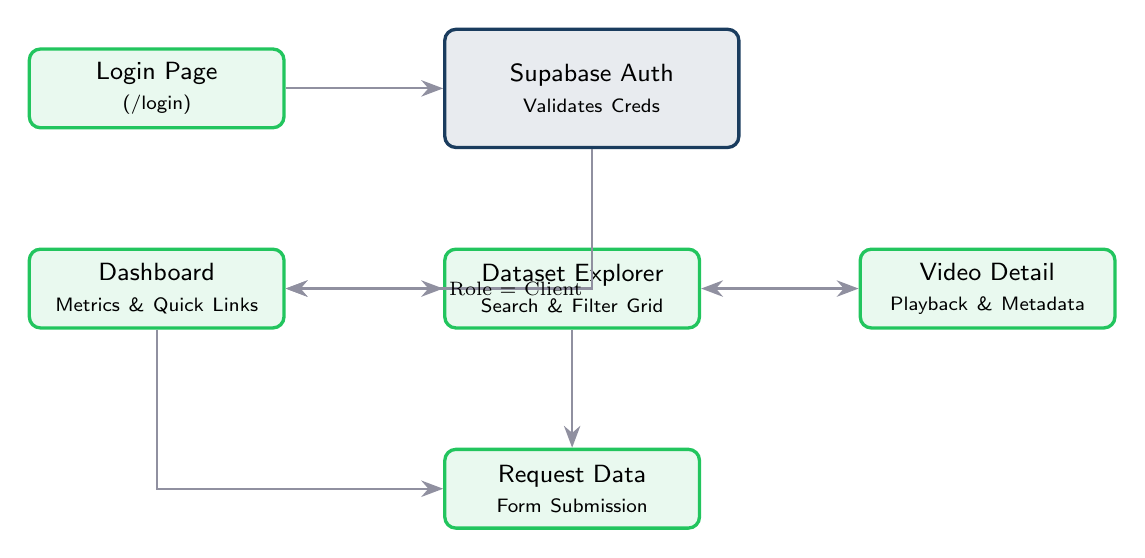
\begin{tikzpicture}[node distance=1.5cm and 2cm]
    \node[client] (login) {Login Page \\ \scriptsize (/login)};
    \node[component, right=of login] (auth) {Supabase Auth \\ \scriptsize Validates Creds};
    \node[client, below=of login] (dash) {Dashboard \\ \scriptsize Metrics \& Quick Links};
    \node[client, right=of dash] (explore) {Dataset Explorer \\ \scriptsize Search \& Filter Grid};
    \node[client, right=of explore] (vid) {Video Detail \\ \scriptsize Playback \& Metadata};
    \node[client, below=of explore] (req) {Request Data \\ \scriptsize Form Submission};

    \draw[arrow] (login) -- (auth);
    \draw[arrow] (auth) |- node[pos=0.75, right, font=\scriptsize] {Role = Client} (dash);
    \draw[biarrow] (dash) -- (explore);
    \draw[biarrow] (explore) -- (vid);
    \draw[arrow] (dash) |- (req);
    \draw[arrow] (explore) -- (req);
\end{tikzpicture}
\end{center}

\section{Next.js UI Component Hierarchy}
\begin{itemize}[label=$\circ$]
    \item \textbf{app/layout.tsx} (Root Layout + AuthProvider Context)
    \begin{itemize}[label=--]
        \item \textbf{app/(client)/layout.tsx} (Sidebar + Top Navbar)
        \begin{itemize}[label=--]
            \item \textbf{app/(client)/dashboard/page.tsx} (Recharts Analytics)
            \item \textbf{app/(client)/collections/page.tsx} (Collection Grid)
            \item \textbf{app/(client)/explorer/page.tsx} (Advanced Sidebar Filters + Video Grid)
            \item \textbf{app/(client)/videos/[id]/page.tsx} (HTML5 Native Video Player)
        \end{itemize}
    \end{itemize}
\end{itemize}

\end{document}
